\documentclass[12pt,a4paper]{article}
\usepackage[margin=25mm]{geometry}
\usepackage{amsmath,amssymb}
\usepackage{booktabs}
\usepackage{graphicx}
\usepackage{hyperref}
\usepackage{xcolor}
\usepackage{enumitem}
\usepackage{microtype}
\usepackage{caption}
\usepackage{array}
\usepackage{longtable}
\usepackage{lineno}

\hypersetup{colorlinks=true,linkcolor=blue!45!black,citecolor=blue!45!black,urlcolor=blue!55!black}
\setlist{nosep}
\emergencystretch=2em
\linenumbers

\newcommand{\workingnote}{%
  \begin{center}
  \fcolorbox{red!55!black}{red!4}{\parbox{0.92\linewidth}{\textbf{Working manuscript.}
  This manuscript reports development and bounded evaluation of a simulation-based safety digital twin.
  Facility-specific ethics and expert review are deployment prerequisites, not
  measured endpoints here; no human-effectiveness claim is made.}}
  \end{center}}

\title{A simulation-based hydrogen refuelling station digital twin
integrating process dynamics, consequence screening and SAGA safety guidance}
\author{\parbox{0.92\textwidth}{\centering
Ugwiyeon Lee\textsuperscript{a}*, Seong-Yun Bae\textsuperscript{a},\\
Hakrae Kim\textsuperscript{a}, Jungsu Lee\textsuperscript{a}, Jinseo Kim\textsuperscript{a}\\
\small \textsuperscript{a}Gas Safety R\&D Institute, Korea Gas Safety Corporation\\
\small 1390 Wonjung-ro, Maengdong-myeon, Eumseong-gun,\\
\small Chungcheongbuk-do 27738, Republic of Korea\\
\small *Corresponding author. E-mail address: lyullee@kgs.or.kr (U. Lee).\\
\small ORCID: U. Lee 0009-0008-8976-5363; S.-Y. Bae 0009-0003-8731-428X;\\
\small H. Kim 0009-0002-5048-3568; J. Lee 0009-0006-9347-453X; J. Kim 0009-0000-2132-6112}}
\date{Working draft: 15 October 2026}

\begin{document}
\maketitle
\workingnote

\begin{abstract}
A simulation-based hydrogen refuelling station digital twin was developed to
connect process dynamics, hazard identification, consequence screening and
staged safety guidance through SAGA, a language-model assistant. The framework
distinguishes observed signals, inferred scenarios, calculated consequences,
requested actions and verified simulated outcomes. Evaluation combined public
experiments, confidential station-side holdouts and public incident records.
Across 12 held-out Type-IV fills, pressure, temperature and state-of-charge
RMSE were 3.841 MPa, 4.833 $^{\circ}$C and 3.850 percentage points. A
same-site recharge forecast achieved 0.184 MPa MAE on 394 holdout cases.
Consequence evaluation identified both bounded successes and failed transfers.
On 34 historical incidents, the SAGA response-structure proxy was 0.760,
compared with 0.401 for alarm-only text. The contribution is an executable,
traceable safety-analysis workflow; complete station control, site-specific
distances and operator effectiveness remain unvalidated.
\end{abstract}

\noindent\textbf{Keywords:} hydrogen refuelling station; digital twin; HAZOP;
consequence analysis; language model; safety decision support

\section{Introduction}
Hydrogen refuelling stations combine high-pressure storage and compression with
rapid changes in flow, pressure and temperature during vehicle filling. A
disturbance can involve several parts of this network: a storage leak changes
inventory and available pressure, isolation changes the connected source, and
residual hydrogen can remain after an emergency-stop command. Safety analysis
must therefore relate an abnormal indication to the physical process, the
possible consequences and the actions available to an operator.

The station decomposition in ISO 19880-1 provides a useful engineering boundary,
while SAE J2601 addresses the vehicle-fuelling protocol \cite{iso19880,saej2601}.
Thermodynamic modelling has established approaches to station-to-vehicle
transfer, cascade optimisation, vehicle-side pressure losses and tank heat
transfer \cite{kuroki2021,rothuizen2013,rothuizen2020,xiao2024}. Consequence
packages such as HyRAM+ provide models of unintended releases and their thermal
and pressure effects \cite{hyram2024,hyram2025}. These capabilities address
different questions. Predicting tank temperature does not establish the accuracy
of an emergency response, and calculating a free-jet consequence does not establish
a safe distance for a particular facility.

The present work addresses the connection between these capabilities. A
conventional alarm identifies a threshold crossing, but leaves the operator to
relate it to concurrent signals, possible causes, equipment isolation and restart
requirements. A language-model explanation can organise this information, yet it
introduces another failure mode if its statements are disconnected from the
current process or if it invents a numerical consequence. An integrated system
needs an explicit account of who owns each state and how every recommendation
can be checked.

This research developed a virtual H70 station coupled to the Safety Analysis
and Guidance Assistant (SAGA). The system links a conserved process model to
virtual instruments, HAZOP rules, consequence calculations and staged response
plans. An operator can then execute a virtual action and inspect its physical
and logical consequences. The research question is whether these links can be
implemented reproducibly and supported by clearly bounded experimental and
incident evidence. The objective is broader than a three-dimensional
visualisation and narrower than a field-qualified automatic safety system.

Three contributions organise the study. First, a shared process state connects
normal operation, fault injection, detection, isolation and consequence
recalculation. Second, HAZOP deviations and incident evidence are converted into
structured response plans with explicit execution and completion conditions;
SAGA explains this context through separate station and sensor interfaces.
Third, a multi-source evaluation distinguishes numerical component performance,
station-side transfer, software correctness and response structure. Negative
results are retained to define the limits of each contribution.

The work uses a simulation-based digital twin: every live sensor and actuator
in the demonstrator is virtual. Confidential operational records are used for
offline calibration and holdout assessment, not as a live connection to a
station. Synchronized station-to-vehicle raw data were not available for a
complete final-system holdout. Accordingly, the paper evaluates components and
integration boundaries separately and makes no claim of SAE-certified control,
validated site separation distances or improved human emergency performance.

\section{Research design and system architecture}
\subsection{System boundary and information ownership}
The reference topology consists of finite tube-trailer supply, a three-stage
compressor, low-, medium- and high-pressure banks, a finite common header,
pre-cooling and two dispenser--hose--vehicle circuits. The circuits retain
independent filling requests and dispatch state. A finite compressor-package
inventory represents gas trapped between isolation boundaries. Storage volumes,
equipment parameters and the visual layout are declared model inputs rather
than an as-built reconstruction.

The Python process service owns the mass, energy, pressure, temperature and
flow states. Virtual sensors expose these states with identity, units,
simulation time, origin and quality. The HAZOP layer evaluates deviations on
those signals. The consequence layer receives a release snapshot; SAGA receives
the resulting process, hazard and consequence evidence. Browser views display
the same job frames and do not independently calculate process dynamics.
Table~\ref{tab:architecture} identifies the responsibility at each interface;
Fig.~\ref{fig:workflow-new} shows the information and virtual-action paths.

\begin{table}[htbp]
\centering\small
\caption{Responsibilities and checkable outputs in the integrated workflow.}
\label{tab:architecture}
\begin{tabular}{>{\raggedright\arraybackslash}p{0.19\linewidth}
                >{\raggedright\arraybackslash}p{0.33\linewidth}
                >{\raggedright\arraybackslash}p{0.39\linewidth}}
\toprule
Layer & Main responsibility & Checkable output \\
\midrule
Process model & Inventory and energy evolution & State trajectories, signed flows and balance residuals \\
Virtual instrumentation & Sample and qualify process evidence & Value, unit, time, origin and quality \\
HAZOP and response logic & Detect deviations and select staged plans & Rule state, supporting signals and completion conditions \\
Consequence analysis & Evaluate a declared release boundary & Calculation status, model inputs, sampled endpoints and uncertainty \\
SAGA & Explain the question using supplied evidence & Grounded answer and claim-limit checks \\
Virtual response & Execute and assess requested actions & Command, motion, feedback, flow confirmation and replay \\
\bottomrule
\end{tabular}
\end{table}

\begin{figure}[htbp]
\centering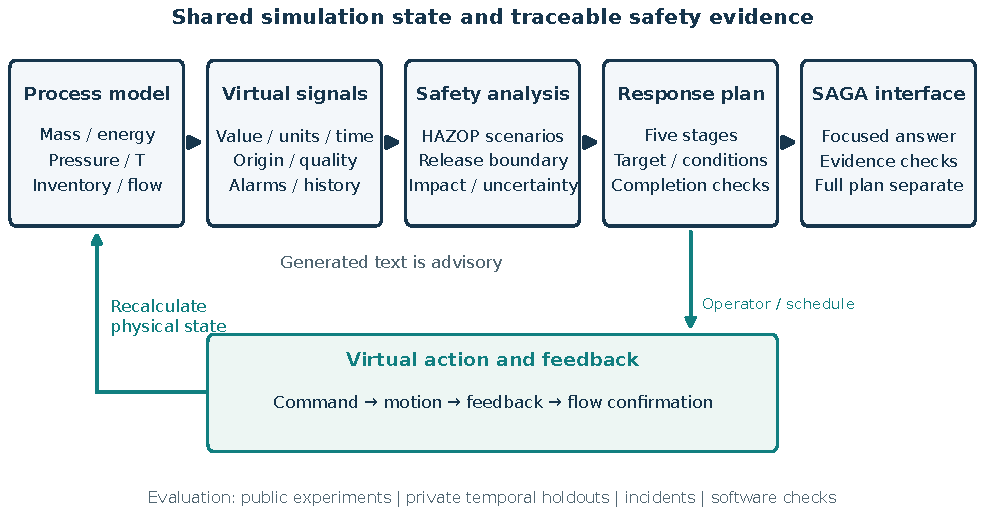
\includegraphics[width=\linewidth]{figures/integrated_safety_workflow.pdf}
\caption{Shared-state workflow. Process dynamics and structured response logic
retain state ownership; consequence results and SAGA explanations carry the
scope of their evidence. Operator-issued or prescheduled virtual commands enter
the action-and-feedback loop shown here.}
\label{fig:workflow-new}
\end{figure}

Three interfaces are kept distinct: the station-level conversation, analysis of
a selected sensor and the standalone SAGA document-search service. This
separation prevents a periodic station report from replacing a user's question
or a general document answer from being presented as current sensor analysis.
The direct digital-twin interfaces use supplied evidence without invoking the
standalone document-search and review sequence on every exchange.

\subsection{Experimental strategy}
The evaluation was organised by observable boundary rather than by a single
system-wide accuracy score. Public filling experiments test vehicle-tank
thermodynamics with measured inlet conditions. Restricted operational traces
test station-side behaviour using disjoint time-ordered records. Public release
experiments test depletion and consequence components. Historical incident
records test response mapping and a deterministic language-output proxy.
Software regressions test whether these interfaces preserve their contracts.

This design separates four evidence roles. Calibration records estimate global
parameters; frozen validation records evaluate the resulting model;
post-outcome diagnostics explain a failure; and contextual sources motivate
scenarios without supplying a numerical score. A source cannot change role
merely because a later model fits it better. Protocols record eligibility,
endpoints, thresholds, input assumptions and code/data hashes where an
outcome-unseen evaluation was possible. Previously accessed records are
explicitly classified as diagnostic or developmental.

\section{Coupled process and virtual safety model}
\subsection{Conserved process states}
For a lumped gas volume $i$, the principal states are hydrogen mass $m_i$,
internal energy $U_i$ and wall temperature $T_{w,i}$. The governing balances are
\begin{align}
 \frac{dm_i}{dt} & = \sum_j \dot m_{ji}-\sum_k \dot m_{ik}, \\
 \frac{dU_i}{dt} & = \sum_j \dot m_{ji}h_{ji}
                  -\sum_k \dot m_{ik}h_i+\dot Q_i, \\
 C_{w,i}\frac{dT_{w,i}}{dt}
     & = UA_{gw,i}(T_{g,i}-T_{w,i})
       +UA_{wa,i}(T_{\mathrm{amb}}-T_{w,i})+\dot Q_{\mathrm{ext},i}.
\end{align}
Pressure and temperature follow from a real-gas property relation,
\begin{equation}
 (p_i,T_{g,i})=\mathcal P_{\mathrm H_2}
       \left(m_i/V_i,U_i/m_i\right).
\end{equation}
The production process calculation uses a versioned property table generated
offline from CoolProp; research evaluators also use direct property calls.
Pressure is consequently an output of inventory and energy, rather than a
prescribed visual trajectory. A leak removes both hydrogen mass and its
outflow enthalpy. Closing an inlet cannot, by itself, stop a breach in the
remaining vessel inventory.

The Type-IV vehicle vessel uses separate gas, liner and composite-shell energy
states. Effective volume and gas-to-liner heat transfer are calibrated globally
across the development fills. The structure captures filling heat input and
delayed heat exchange without resolving spatial gas mixing. Where public vessel
geometry is unavailable, volume is scaled from 0.122 m$^3$ per 4.7 kg nominal
capacity. The use of an effective geometry is carried into the interpretation of
temperature and SOC errors.

Flow restrictions use an effective opening area and discharge coefficient.
The research real-gas restriction calculation evaluates the accessible
isentropic mass flux,
\begin{equation}
 G(p)=\rho(p,s_0)\sqrt{2[h_0-h(p,s_0)]},\qquad
 \dot m=C_d A_{\mathrm{eff}}G_* ,
\end{equation}
where $G_*$ is the maximum accessible flux between downstream and upstream
pressure. The coefficient and aperture describe a particular boundary; they
cannot absorb an unknown pipe network without changing the model's meaning.

\subsection{Compression, cascade dispatch and filling control}
The compressor uses a quasi-steady positive-displacement representation with
suction-density, efficiency and staging assumptions. Interstage cooling and
pre-cooling provide the thermal boundary for storage recharge and dispensing.
The vehicle controller uses a sampled pressure-ramp request, flow limitation,
valve dynamics and protective termination. It represents an APRR-style control
boundary, with no proprietary SAE J2601 lookup tables or MC Formula claim.

Cascade selection and recharge are stateful. The selected dispensing bank
progresses through the available pressure levels, while recharge uses a lower
restart boundary and an upper stop target. This hysteresis avoids instantaneous
switching around a single pressure threshold. The high-bank restart band is
informed by a disclosed same-site development diagnostic; it is not an approved
operating limit. Normal stop targets, relief settings and protective trips are
separate inputs so that removing a normal operating target does not silently
remove a protection layer.

\subsection{Detection and HAZOP evaluation}
The versioned HAZOP catalogue connects process nodes to pressure, temperature,
flow, gas and flame signals. Each rule retains its condition, persistence,
operating-mode qualification and recovery behaviour. The current catalogue has
214 executable simulation rules. This is implementation coverage: it does not
establish 214 independently validated hazard detectors.

Mode qualification is essential. Zero flow is expected when a dispenser is
idle; it is potentially abnormal only when a transfer is requested and the
necessary operating conditions are satisfied. A detector below its threshold
can also coexist with a retained alarm. The runtime therefore distinguishes a
current observation, an active rule, a latched history and an injected physical
fault. Missing or stale input is represented through quality and rule state,
rather than being converted to a reassuring numerical zero.

Scenario grouping combines related indications while preserving competing
interpretations. A storage gas alarm, pressure loss and an observed release can
support one release scenario; a threshold crossing alone does not establish a
breach size, ignition or structural failure. A fire scenario has a virtual
flame-detection path and separate exposure logic. Detector concentrations are
labelled by their calculation origin, including a proxy origin where applicable.
They are not treated as spatially validated field measurements.

\subsection{Executable actions and completion conditions}
The virtual action model distinguishes command issue, valve motion, position
feedback and measured flow cessation. Stuck position, internal leakage,
partial closure and feedback error can therefore produce a failed action even
after a close command has been accepted. The model also provides virtual ESD,
bank venting, ventilation, cooling, access restriction and evacuation tracking.
The latter are training states; their implementation does not solve pedestrian
movement, ventilation CFD or a physical fire-suppression process.

Recovery follows a separate sequence: source repair, leak/functional checks,
purge and repressurisation proxies, then restart approval. A new incident
invalidates earlier recovery records. A numerical value returning below its
alarm threshold does not by itself complete recovery. Likewise, source
termination after a confirmed immediate-stop sequence is distinguished from
residual-hazard clearance. The current virtual clearance rule requires three
consecutive samples with negligible release, less than 0.2 vol\% H$_2$,
usable detector quality and no ventilation fault. These values are exercise
settings, not facility re-entry criteria.

Every action is followed by process-state evolution and updated release,
detector and consequence fields. The framework can schedule paired virtual
runs with identical initial states and faults, comparing no action, isolation,
ESD and ESD with isolation/ventilation. The feature supplies an experimental
instrument for future response comparisons. No reduction in real accident
severity is inferred from its availability or from a completed software test.

\section{Consequence analysis and SAGA integration}
\subsection{Release snapshots and consequence endpoints}
HyRAM+ 6.1 is connected through a versioned adapter. A calculation request
declares the source pressure and temperature, aperture, discharge assumptions,
orientation and observation geometry. An active modelled release and a
sensor-based hypothetical release are separate request origins. The latter
supports conditional analysis but does not establish that a leak exists or that
its aperture has been identified.

The outputs distinguish directional 4 vol\% hydrogen plume extent from sampled
thermal and overpressure criteria. For thermal radiation and unconfined
overpressure, the displayed extent is derived from configured observation points
exceeding 5 kW m$^{-2}$ or 5 kPa, respectively. It is a sampled screening
extent, not an exact continuous contour. A missing crossing remains unestablished;
it is not replaced by a default 1 m radius. Visible flame length, plume extent,
sampled criterion crossing and the equipment footprint remain different fields
throughout the API and visualisation.

Calculation status and time accompany the consequence result. A reused result
retains its snapshot provenance; a failed backend call cannot be replaced by a
language-model estimate. The dynamic display can compare equipment-relative
hazard indices, but its 0--100 score has no calibrated annual frequency or
individual-risk interpretation. Three-dimensional overlays are explanatory
graphics around equipment, not a numerical mesh of the release field.

\subsection{Uncertainty and permitted use}
An on-demand sensitivity function perturbs declared pressure, temperature,
aperture and discharge-coefficient bounds with a reproducible stratified
ensemble. The default bounds are $\pm3\%$, $\pm3$ K, $\pm10\%$ and
$\pm12\%$, respectively, with 24 samples and seed 731; the implementation caps
the ensemble at 128. It reports P05/P50/P95 of available consequence fields and
input--output correlations. These are percentiles of the assumed sensitivity
ensemble. They are neither experimental confidence intervals nor a calibrated
joint probability distribution of station failures.

Each result also carries model identity, validation scope, input quality,
uncertainty status and permitted uses. Current component evidence permits
screening advice with usable inputs while blocking autonomous actuation based
on the consequence result. Deterministic protective logic operates through its
own path; an LLM explanation cannot override it. This makes the validation
boundary a runtime property of the result rather than a warning confined to
the paper.

\subsection{Structured response plans}
Response plans use five stages: situation confirmation, immediate action,
stabilisation, checks before restart and prevention. A step identifies its
target equipment, virtual command where available, supporting conditions and
completion evidence. Simultaneous compatible indications are consolidated into
a response sequence so that the operator does not receive a separate full
emergency procedure for every threshold. Conflicting evidence and unavailable
inputs remain explicit.

For normal operation, the interface presents monitoring and preventive controls.
For abnormal operation it adds the relevant emergency sequence and calculated
consequences. A plan is retained as structured deterministic data outside the
generated answer. This allows a focused conversational response without
discarding the full procedure, and permits a step to be linked to a simulation
command whose outcome can subsequently be inspected.

\subsection{Direct assistance and document-grounded knowledge}
SAGA-PY provides standalone document retrieval as well as the two dedicated
digital-twin interfaces. Its document service uses SQLite lexical search and a
local hash n-gram index, followed by evidence selection and citation checks.
The licensed local corpus is not distributed with the public code. A general
document answer and a current-state analysis therefore have different evidence
contracts and should not be pooled as one validated capability.

The twin uses a direct-answer configuration. The current sensor or user
question is prioritised together with quality, active and retained alarms,
release evidence and available consequence results. A compact evidence
projection is sent to the provider; the full manifest remains in the local API
with a digest linking the two. Raw confidential traces and facility identifiers
are not provider context. The main assistant is question-focused, whereas the
sensor assistant receives the selected sensor and related process evidence.
Periodic analysis is a distinct request type and display path.

The generated answer is checked for unsupported value--unit claims and claims
that exceed the registered validation scope. A numerical guard is a limited
syntactic/grounding safeguard: it cannot establish that a qualitatively worded
recommendation is correct. Streaming improves presentation responsiveness but
does not change the underlying physical result or the evidential status of the
answer. Model identity and configuration must be recorded when comparing runs.

\section{Data and evaluation methods}
\subsection{Public filling data and station-side records}
Five checksum-verified H2Protocol/Powertech archives supplied 36 Tables Method
fills \cite{schneider2014}. A pre-model mass-closure screen accepted an
integrated measured-flow to SOC-implied inventory ratio of 0.8--1.2. One case
was excluded at 1.428. Every third laboratory test formed the 12-case validation
set; 23 admissible cases were used for fitting two global multipliers. The
experimental time base was retained without fitted shifts or dynamic time
warping. A disclosed parser amendment removed an isolated startup pulse from
development case L29; the tank fit and all quoted tank results use the corrected
normalisation.

For each case, pressure, gas temperature and density-based SOC were scored
separately using
\begin{equation}
 \mathrm{RMSE}(y)=\sqrt{\frac{1}{n}\sum_{k=1}^n
       [y_k^{\mathrm{predicted}}-y_k^{\mathrm{measured}}]^2}.
\end{equation}
Case means were bootstrapped with 10,000 replicates and seed 2601. Samples within
a fill were not treated as independent experimental replicates.

Confidential operational traces were assessed offline using calibration and
disjoint time-ordered holdout partitions. Public outputs contain de-identified
counts, relative-time results and approved aggregate errors. They exclude
operator, facility, location, manufacturer, exact dates, original tags and raw
rows. This is same-site temporal transfer, with no independent-site claim.
Pressure-boundary replay, medium/high cascade order and short-horizon recharge
pressure forecasting were evaluated separately. A recharge-dwell rule and
lifecycle-counter alignment provide retained negative controls on broader
interpretation.

The forecast is an empirical adjunct, not a calibration of the conserved
station model. Each trace was split 70/30 chronologically before extracting
non-overlapping 40 s windows. An observed 10 s loaded-compressor prefix selects
the responding bank; a bank-specific robust gain predicts the following 30 s
pressure increment. Target selection uses prefix data only. The earlier
partition fits the median ratio of future to prefix pressure rates, clipped
to $[-1,3]$. Persistence and uncalibrated prefix-rate extrapolation are
comparators. Eligibility requires continuous loaded operation, gaps no longer
than 2.5 s and a prefix rise of at least 0.10 MPa with a 1.5 dominance ratio.
The primary screens require median/P90 error no greater than 0.5/1.5 MPa,
at least 20\% MAE improvement over persistence, at least 90\% direction
agreement and no more than 50\% gain shift. This conditional forecast does
not predict an unknown compressor-state transition.

A supplementary public intake contained 15 MetHyTrucks workbooks and 58,440
synchronised samples \cite{methytrucksgroupa2026,methytrucks2026,
methytrucksgroupc2026}. Metadata limitations, sampling-system rather than
vehicle boundaries and prior outcome access restrict these records to
descriptive closure and development diagnostics. They are not added to the
frozen Type-IV validation population.

\subsection{Release, consequence and software verification}
The ambient PRESLHY E3.1 evaluation fixed model and protocol hashes before
numerical workbook access \cite{preslhy2023}. Its 22 eligible cases span 0.5,
1, 2 and 4 mm apertures in a 2.815 L vessel. The frozen model was adiabatic,
with instantaneous opening and $C_d=0.8$. A case required pressure NRMSE
$\leq10\%$ of initial absolute pressure and half-gauge-pressure-time error
$\leq20\%$; the aggregate pass threshold was 70\%. Numerical failures were
retained. Wall heat transfer was subsequently developed on those consumed
records and tested on E5.1 \cite{preslhye5}. Ambient Part-B used its own
separately frozen depletion configuration \cite{preslhypartb}.

Transfer was also examined with INERIS/CEA high-pressure releases, Sandia/SRI
mass-flow and pressure-decay traces, and the small-inventory Ekoto release
\cite{proust2011,schefer2006,schefer2007,ekoto2012}. Digitised curves retained
their extraction provenance and declared uncertainty where available. Separate
protocols fixed the relevant flow, pressure and half-time screens before the
respective comparisons; no universal threshold was imposed retrospectively
across physically different experiments.

For the immediately ignited vented-enclosure component, four previously viewed
cases were assigned to development and 27 untouched cases to a frozen holdout
\cite{lach2021ignited}. A species/energy balance used measured mass-flow
histories and common reported coefficients without case-specific fitting. The
primary decision required at least 20 cases and at least 80\% with peak-pressure
absolute error $\leq2$ kPa. A separate 44-case delayed-ignition rank screen
tested whether pressure/nozzle inputs preserved severity ordering after
instrumentation and geometry-related stratification \cite{wskbij2026}.

HyRAM+ verification compared installed source hashes with public v6.1 sources,
ran 47 upstream physics tests and compared three production-adapter cases
against direct public-API calls. Translation tolerance was $10^{-12}$ relative
and $10^{-9}$ absolute. These are package and interface checks, distinguished
from independent experimental validation of the station configuration.

\subsection{Incident mapping and SAGA comparison}
The public HRS subset of HIAD 2.2 supplied 34 historical incidents, 33 with an
emergency-action, lesson or corrective field \cite{hiad2026}. Scenario mapping
and virtual command coverage were evaluated separately from generated-answer
quality. Public KHK reports supplied an additional accident-provenance check
\cite{khk2026}; incident prose did not set physical model parameters.

The retrospective language comparison used all 34 events. Historical
emergency-action, lesson and corrective fields were withheld from model-visible
context. One direct SAGA answer per event was compared with deterministic
alarm-only text under the archived English, 900-token configuration. The proxy
was fixed before cohort answer collection, but the category taxonomy and
references had already been used in development. It is consequently a
development benchmark rather than an independent prospective holdout.
The archived run records Groq and model identifier
\texttt{qwen/qwen3.8-27b}; each event contributes one generated answer.

For event $e$, the proxy is
\begin{equation}
 S_e=\tfrac12(R_e+C_e),
\end{equation}
where $R_e$ is expected coarse action-category recall and $C_e$ is coverage of
the five response stages. The eight categories span isolation, detection,
fire/cooling, evacuation, communication, inspection/repair, procedural controls
and ventilation/purge. A paired event-level bootstrap used 10,000 replicates and
seed 20261008. A subsequent audit evaluated reference precision/F1, additional
categories and word count on saved guarded answers. That audit is explicitly
post-outcome and used a different output revision.

No operator trial or expert correctness rating was conducted. The comparison
tests structure and coarse lexical alignment; it cannot isolate the effect of
the LLM from the richer context and response templates supplied to it. Historical
reports are also incomplete references, so an additional category is not
automatically an unsafe recommendation.

\section{Results}
\subsection{Vehicle-boundary thermodynamics}
The fitted effective-volume and gas-to-liner multipliers were 1.05273 and
31.46066. Table~\ref{tab:tank-new} gives case-mean errors and bootstrap intervals.
The 12 validation fills produced mean RMSE of 3.841 MPa, 4.833 $^{\circ}$C
and 3.850 SOC percentage points. Figure~\ref{fig:tank-new} shows the joint
pressure/temperature comparison; Fig.~\ref{fig:cases-new} exposes the between-fill
variation hidden by the means.

\begin{table}[htbp]
\centering\small
\caption{Type-IV model errors; parentheses are case-bootstrap 95\% intervals for the mean.}
\label{tab:tank-new}
\resizebox{\linewidth}{!}{%
\begin{tabular}{lrrrr}
\toprule
Set & Fills & Pressure RMSE (MPa) & Temperature RMSE ($^{\circ}$C) & SOC RMSE (points) \\
\midrule
Calibration & 23 & 4.529 (3.237--6.126) & 7.889 (6.072--9.870) & 4.455 (3.517--5.455) \\
Validation & 12 & 3.841 (2.507--5.835) & 4.833 (3.707--6.113) & 3.850 (2.921--4.909) \\
\bottomrule
\end{tabular}}
\end{table}

\begin{figure}[htbp]
\centering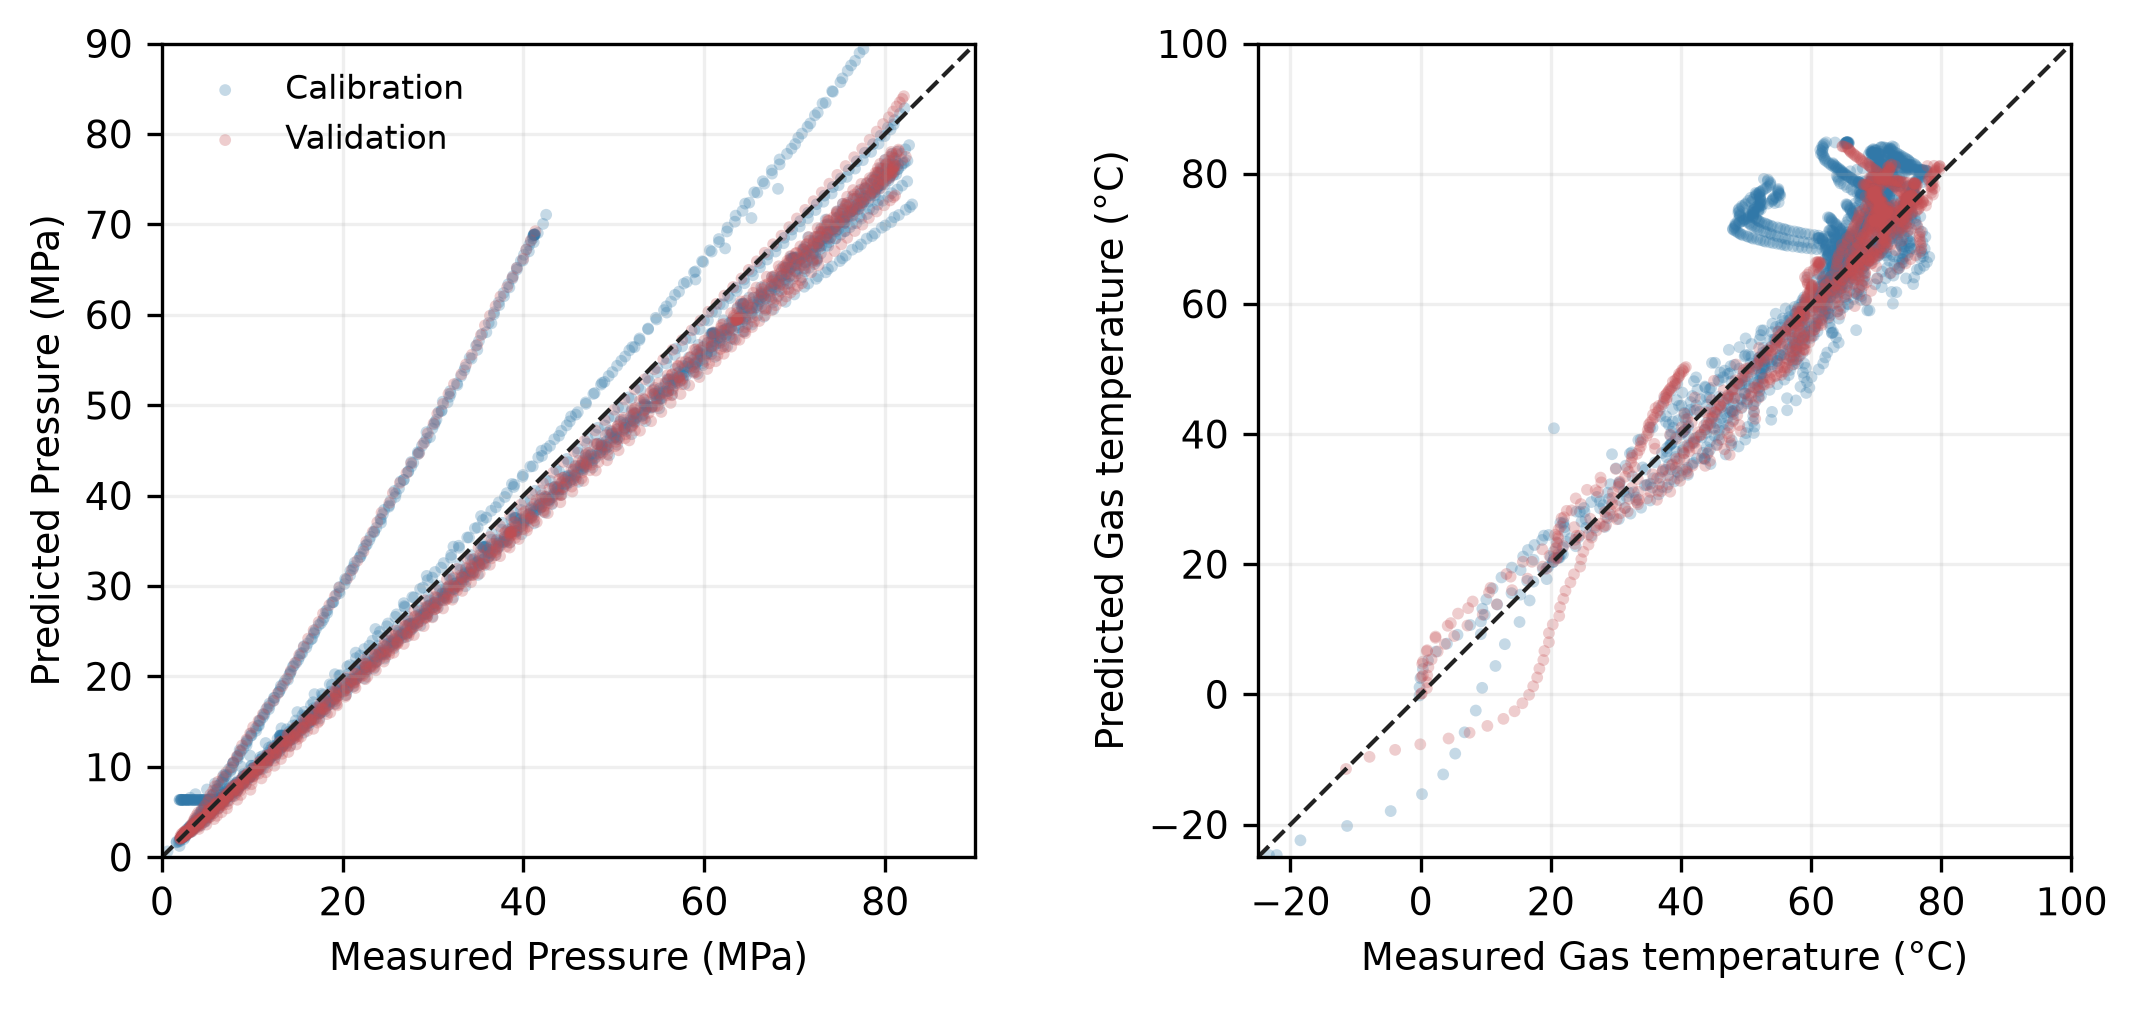
\includegraphics[width=\linewidth]{figures/tank_parity.png}
\caption{Measured-boundary Type-IV pressure and gas-temperature predictions on
the experimental clocks. The dashed line is equality.}
\label{fig:tank-new}
\end{figure}

\begin{figure}[htbp]
\centering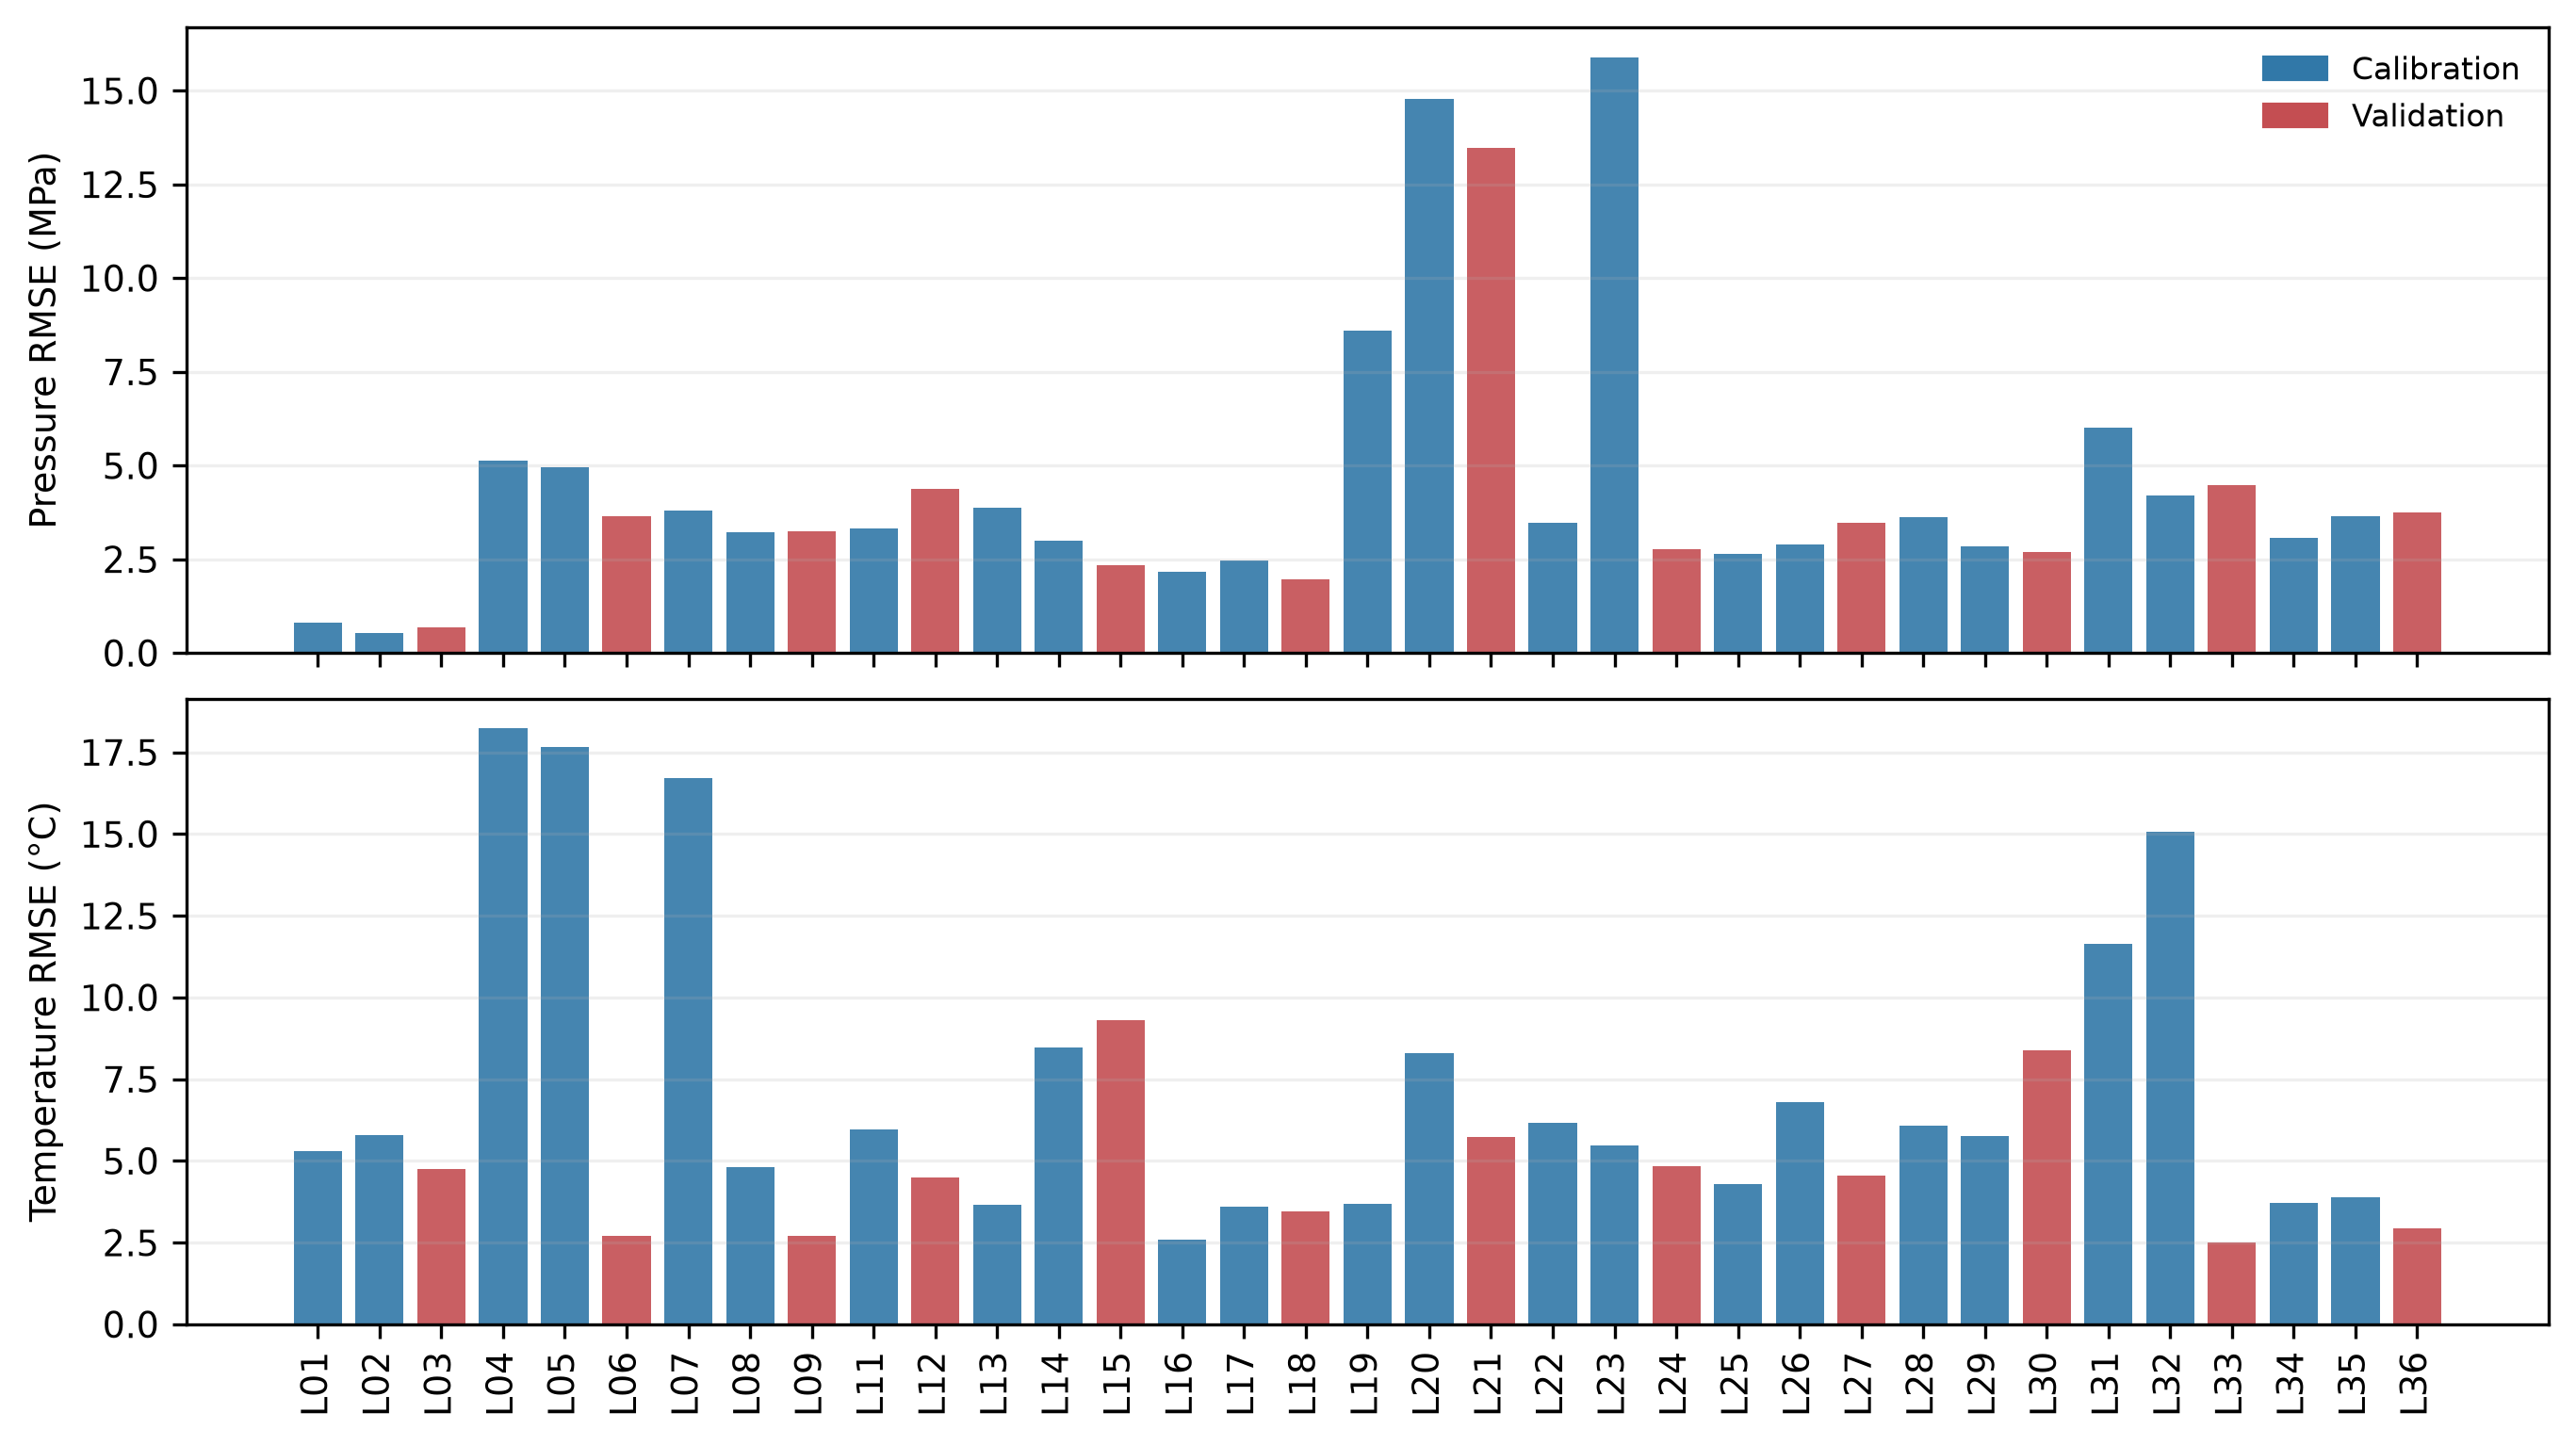
\includegraphics[width=\linewidth]{figures/tank_case_rmse.png}
\caption{Fill-level errors with frozen validation cases separated from calibration.
The pre-model mass-closure exclusion has no bar.}
\label{fig:cases-new}
\end{figure}

Lower validation than calibration means do not establish universal
generalisability. The large heat-transfer multiplier is an effective correction,
and first-order optimality of 3115.9 despite successful optimiser termination
indicates incomplete parameter identification. A prospective Type-III transfer
passed pressure at 0.943 MPa RMSE but failed temperature at 19.179 K RMSE.
The underlying experiment has a distinct vessel and heat-transfer boundary
\cite{andreasen2026archive,couteau2025flow}.
Together, these findings support the tested Type-IV boundary while exposing a
thermal-transfer limitation.

The supplementary MetHyTrucks audit detected 18 sessions. Nine had changing
scale mass and eight of those nine met the descriptive 0.8--1.2 flow--mass
closure screen (median ratio 1.003). Unchanged-scale sessions were unscored.
Neither this closure result nor a successful sampling-system replay validates
vehicle-filling control.

\subsection{Station-side holdouts and full-loop transfer}
The restricted-data assessment supports several specific station-side results
(Table~\ref{tab:station-new}). The 394-case recharge-pressure holdout gave
0.184 MPa MAE and 0.529 MPa P90 absolute error; medium/high cascade pairs had
a 94.38\% sequential fraction among evaluated pairs. Coverage and event
definitions are part of these results: the cascade fraction does not represent
all station events, and a short-horizon pressure forecast is not a compressor
capacity or complete charging-cycle prediction.

Persistence MAE was 0.656 MPa and uncalibrated prefix extrapolation MAE was
0.196 MPa. The calibrated surrogate improved MAE by 71.9\% against
persistence but only 5.8\% against prefix extrapolation. Most of the benefit
therefore comes from using the observed pressure trend rather than the fitted
gain. Medium/high holdout MAE was 0.116/0.227 MPa across 151/243 cases;
the overall positive-direction fraction was 94.9\%. These results remain
conditional on the eligible loaded-compressor windows.

\begin{table}[htbp]
\centering\small
\caption{Confidential same-site temporal holdouts. No raw or identifying records are disclosed.}
\label{tab:station-new}
\begin{tabular}{>{\raggedright\arraybackslash}p{0.25\linewidth}
                >{\raggedright\arraybackslash}p{0.23\linewidth}
                >{\raggedright\arraybackslash}p{0.43\linewidth}}
\toprule
Endpoint & Holdout population & Retained result \\
\midrule
Pressure-boundary replay & 30 points, 1,755 s & Replay completed; bounded boundary evidence \\
Medium/high cascade order & 3,664 pairs & 94.38\% sequential; pair coverage 70.39\% \\
Recharge-pressure forecast & 394 cases & MAE 0.184 MPa; P90 error 0.529 MPa \\
Lifecycle-counter alignment & Counter/pressure holdout & Recall 19.60\%; pressure precision 90.27\%; negative \\
Recharge time dwell & 32 completed restarts & Holdout minimum 176.0 s below fitted 290.0 s; negative \\
\bottomrule
\end{tabular}
\end{table}

The dwell rule was disabled after its failed temporal transfer. A separate
post-outcome analysis of 124 completed stop/restart cycles gave a median
high-stage pressure drop of 4.555 MPa. The rounded 4.5 MPa restart band is
therefore an evidence-informed development setting, with no untouched holdout
claim. The pressure forecast and cascade checks remain separate from that
setting and from the failed lifecycle-counter interpretation.

Complete station-to-vehicle transfer was substantially harder. An earlier
prospectively frozen MC Default controller configuration passed 0/8 joint
screens, with mean pressure, temperature and SOC RMSE of 15.862 MPa,
13.230 $^{\circ}$C and 18.082 points. These experiments supplied a
pressure--time schedule, whereas the frozen implementation accepted an
endpoint-equivalent constant ramp. The result therefore tests that disclosed
approximation and historical configuration, not a faithful MC Formula or the
final implementation.

Subsequent development corrected parsing, nominal-pressure handling,
anti-windup, cooling-class protection and cascade dispatch. Corrected development
and already-inspected comparison sets still passed only 1/8 and 2/11 joint
screens. Their mean errors were 6.602/4.530 MPa, 11.428/7.819 $^{\circ}$C
and 7.297/4.625 SOC points, respectively. The consumed prospective set was
not used to issue a new positive final-system decision. Thus a successful
measured-inlet tank model coexists with unresolved controller and boundary
transfer errors.

\subsection{Release and consequence applicability}
The independent component results are mixed (Table~\ref{tab:release-new}). The
frozen ambient E3.1 source model passed 11/22 joint screens, below its 70\%
criterion; six high-pressure cases retained thermophysical-domain failures.
Adding wall thermal inertia and real-gas discharge removed those failures and
passed 20/22 consumed cases, but this developmental improvement did not transfer
to an eligible, sufficiently large E5.1 holdout. Only three cases met its
primary eligibility definition and two passed; the protocol required at least
four. Ambient Part-B passed 3/5, also below 70\%.

\begin{table}[htbp]
\centering\small
\caption{Release/consequence endpoints retained by experiment. Joint decisions
use their original protocols; they are not pooled as a single accuracy.}
\label{tab:release-new}
\begin{tabular}{>{\raggedright\arraybackslash}p{0.31\linewidth}
                >{\raggedright\arraybackslash}p{0.22\linewidth}
                >{\raggedright\arraybackslash}p{0.38\linewidth}}
\toprule
Experiment and endpoint & Joint result & Main interpretation \\
\midrule
PRESLHY E3.1 ambient depletion & 11/22; failed & Adiabatic source insufficient across tested groups \\
E5.1 revised-source transfer & 2/3 eligible; insufficient & Minimum sample and pass criterion unmet \\
Ambient Part-B depletion & 3/5; failed & Timing errors despite passing pressure screens \\
INERIS/CEA near 90 MPa flow & 0/3 aperture series & Diameter/apparatus transfer unsupported \\
Sandia/SRI 2006 flow & Joint screen failed & NRMSE 5.83\%; median and half-time errors failed \\
Sandia/SRI 2007 pressure & Joint screen failed & NRMSE 11.58\%; half-time error 6.51\% passed \\
Ekoto small-inventory flow & All three screens passed & NRMSE 3.84\%; bounded 13.45 MPa, 3.63 L source \\
Unignited enclosure peak & 7/10; failed & Below frozen 80\% aggregate criterion \\
Immediately ignited enclosure peak & 27/27 passed & MAE 0.672 kPa; maximum error 1.796 kPa \\
Large-scale delayed-ignition rank & Controlled screens failed & Pooled association did not survive stratification \\
\bottomrule
\end{tabular}
\end{table}

The Ekoto transfer passed all frozen mass-flow screens, including 12.79\%
median absolute percentage error and 6.07\% half-peak-time error. Its short,
small-inventory release and independently specified coefficient distinguish it
from the longer or higher-pressure failed transfers. It therefore provides a
bounded positive result, rather than a correction factor for every apparatus.

For the immediately ignited enclosure, all 27 cases met the primary 2 kPa
peak-pressure screen. Secondary timing and trace-NRMSE screens passed 21/27
and 26/27. The measured source-flow boundary is important: this validates the
enclosure pressure-peak calculation under the tested geometry, not source
depletion upstream of that boundary. The unignited enclosure passed 7/10,
below its distinct frozen 80\% threshold \cite{lach2020}.

The delayed-ignition archive further demonstrates why geometry matters. Across
44 cases, pooled Spearman correlation was 0.572. After stratification, correlation
was $-0.023$, concordance 0.421 and top-third recall 0.294, below their
0.45/0.65/0.50 criteria. Predictions spanned only 22.091--22.740 kPa against
measured maxima of 0.220--235.390 kPa. Source pressure and aperture alone did
not preserve controlled severity ordering; this result is not converted into
a station explosion-distance claim.

\subsection{Software translation and executable response coverage}
The installed HyRAM+ source matched the public v6.1 source over 38 Python files.
All 47 selected upstream tests, comprising 803 subtests, passed; all three
production-adapter parity cases met the specified numerical tolerance. The
low-bank 1 mm, cold mid-bank 2 mm and high-bank 3 mm cases returned directional
4 vol\% plume extents of 4.339, 11.382 and 17.224 m. These are example
model outputs under declared inputs, not measured site boundaries.

All 34 HIAD cases mapped to registered response families. Replay covered 29
through direct process representations, four through a compressor proxy and
one structural-damage case through response logic only. The five
active-response categories produced 72 event--category obligations with virtual
commands. Ten family templates executed 52 commands with completion feedback.
The counts establish mapping and execution coverage, not independent
effectiveness of every action. KHK citation-based metadata provided a separate
check across 23 reports and 26 incident codes; eight registered response
recipes passed their integration checks.

An archived full Python regression run reported 1,650 passed, no failures and
no skipped tests, with 23 warnings. It is an implementation snapshot at the
recorded code revision, not a physical-accuracy percentage. Current extensions
also provide partial-closure, stale/dropout and residual-hazard checks, plus
paired-run and sensitivity interfaces. Their implementation status is kept
separate from the earlier empirical evaluations and does not enlarge those
experimental samples.

\subsection{SAGA response structure and information burden}
The archived 34-event comparison favoured SAGA on its declared machine proxy
(Table~\ref{tab:saga-new}). Mean category recall was 0.524 versus 0.189 and
stage coverage 0.982 versus 0.600. The mean proxy difference was 0.360 with
a paired bootstrap interval of 0.309--0.411. The first run flagged unsupported
value--unit claims in 3/34 SAGA answers; a later guarded rerun reduced the
flagged count to 0/34. That rerun is a post-outcome engineering correction,
not the original benchmark result or evidence that all unsafe statements were
removed.

\begin{table}[htbp]
\centering\small
\caption{Original retrospective HIAD comparison, one answer per event.}
\label{tab:saga-new}
\begin{tabular}{lrr}
\toprule
Metric & Alarm-only & SAGA \\
\midrule
Events & 34 & 34 \\
Mean expected-category recall & 0.189 & 0.524 \\
Mean five-stage coverage & 0.600 & 0.982 \\
Mean response-structure proxy & 0.401 & 0.760 \\
Answers with unsupported numeric flags & 0 & 3 \\
Failed calls & 0 & 0 \\
\bottomrule
\end{tabular}
\end{table}

The saved guarded-output audit on 33 reference-evaluable events exposes a
trade-off. Reference F1 was 0.564 versus 0.281, while precision was
0.680 versus 0.697. Mean word count rose from 28.1 to 140.5 and mean
non-reference category count from 0.303 to 0.970. Greater coverage therefore
came with more information to process. The display design uses a focused answer
with the deterministic full plan separately available; this is a design
response to the burden, not a demonstrated reduction in operator workload.

\section{Discussion}
\subsection{What the integrated workflow adds}
The principal result is the connection between a safety statement and its
checkable process context. A gas alarm can be displayed together with its
quality, a possible release source, a declared consequence request, applicable
isolation commands and the measurements needed to confirm success. The next
simulation sample then updates the process instead of merely marking the
procedure complete. This gives the demonstrator a causal training structure
even where the quantitative physical fidelity remains limited.

Consider a storage-vessel leak. Isolating connected inlet/outlet paths changes
the connected inventory, but the remaining vessel can continue to release.
Ending the source input after an exercise stop sequence still leaves a separate
residual-hazard state. A requested valve closure can fail its feedback or
flow condition. Keeping these distinctions visible prevents a textual answer,
accepted command or cleared badge from serving as its own evidence of safety.
This is the rationale for combining physical state, HAZOP, consequence screening
and staged guidance within one traceable workflow.

The contribution is not a new universal release correlation or an independently
validated autonomous safety policy. It is an integration method that preserves
the evidence boundary of its components. The direct SAGA interface adds
question-specific explanation to this structure; the standalone retrieval
service supplies a separate document-knowledge capability whose citation
quality requires its own evaluation.

\subsection{Interpreting the physical evidence}
The strongest filling result is the measured-boundary Type-IV model. Supplying
the experimental inlet flow and temperature removes controller and upstream
uncertainty from that test. It is therefore compatible with a negative
station-to-vehicle result: an adequate downstream model can be driven by an
inadequate upstream schedule. The large effective heat-transfer correction and
failed Type-III temperature transfer warn against interpreting an aggregate
temperature error as an identified material parameter.

The confidential data add a different form of evidence. A useful same-site
recharge-pressure forecast and a largely sequential cascade pattern help
ground station-side behaviour, but do not provide missing vehicle inlet,
controller or receptacle measurements. The failed dwell and counter checks
show that temporal event interpretation cannot simply be inferred from a
plausible pressure trajectory. These records improve the realism of bounded
operational assumptions without making the public component and confidential
station samples interchangeable.

Release results are similarly boundary-dependent. Vessel-wall heat and
line/manifold inventory matter for depletion, while the successful enclosure
pressure model is driven by measured source flow. HyRAM+ adapter parity removes
one integration uncertainty, but cannot repair an incorrect release boundary.
For this reason the interface preserves both the point calculation and the
input/domain flags. Failure to reproduce geometry-controlled explosion ranking
also precludes converting a visually convincing overlay into a validated
equipment hazard zone.

\subsection{Meaning and limits of the SAGA evaluation}
The retrospective comparison demonstrates that the linked configuration
produced more of the selected action categories and response stages than the
compact alarm baseline. It does not demonstrate that a language model selected
the safest action. Richer context, deterministic templates and longer output
are all plausible contributors; the study contains no factorial ablation that
separates them. A single answer per event also leaves provider/model
stochasticity unmeasured.

The unsupported-numeric findings motivate a guard, while the precision and
length findings motivate prioritisation. Neither supplies a complete safety
assurance argument. A clinically or industrially consequential omission can
receive a high lexical score, and a prudent action absent from a short
historical report can lower measured precision. Expert assessment of action
correctness, facility-specific review and operator testing are therefore
prerequisites for operational deployment, outside the endpoints measured here.
KGS-collected, de-identified research material and AI-assisted organisation
informed the preliminary evidence and response resources; they do not replace
that review.

\subsection{Limitations and reproducibility}
All instruments, interventions and scene effects are simulated. Geometry,
weather, occupancy, heat-transfer coefficients, compressor performance and
most actuator failure parameters remain scenario assumptions. Spatial detector
response and ventilation are not independently validated at station scale.
Detailed structural failure, realistic evacuation timing, spray/fire interaction
and full probabilistic QRA are beyond the demonstrated physical scope.

No openly reusable synchronized station-to-vehicle raw cohort with the required
controller, thermal and vehicle channels was identified. The full-loop result
therefore remains a disclosed negative transfer diagnostic rather than a
primary final-system accuracy claim. Sources containing plots, aggregate
operating summaries or inaccessible raw files were not promoted to substitute
holdouts. Future validation should prioritise a defined apparatus and endpoint
with complete units, geometry and common-time measurements, rather than an
ever-larger collection of loosely compatible records.

Public scripts, hashes and result manifests permit inspection of the reported
comparisons, while restricted raw records remain owner-controlled. Readers can
reproduce the public numerical experiments and software interfaces subject to
third-party access and licensing. They cannot independently reconstruct private
station traces from the published aggregates. The release-network candidate,
paired intervention interface and bounded sensitivity function are available
for future tests; no unreported empirical success is inferred from them.

\section{Conclusions}
This study developed a simulation-based hydrogen-station safety digital twin
that links process dynamics, HAZOP deviations, consequence calculations and
SAGA guidance to executable virtual responses. Its defining feature is the
preservation of distinctions between a signal, an inferred scenario, a
calculated consequence, an action command and confirmed simulated completion.

Evaluation supports several bounded results: measured-boundary Type-IV
prediction at 3.841 MPa pressure and 4.833 $^{\circ}$C temperature RMSE;
same-site recharge-pressure forecasting at 0.184 MPa MAE; a 27-case
ignited-enclosure peak-pressure result at 0.672 kPa MAE; and verified HyRAM+
translation. Negative controller, depletion and geometry-transfer results
define where those findings do not apply.

SAGA increased retrospective response-structure coverage, with a proxy of
0.760 against 0.401 for alarm-only text, while a separate audit exposed longer
answers and additional action burden. The combined outcome is a reproducible
research and training framework with traceable numerical and procedural
boundaries. Field deployment requires the facility-specific measurement,
HAZOP, expert and operational evaluations appropriate to the intended use.


\section*{Data and code availability}
The digital-twin source, evaluation scripts, result manifests and documentation
are available at \url{https://github.com/lyullee/hydrogen-station-sim}, archived
as \href{https://doi.org/10.5281/zenodo.23084421}{10.5281/zenodo.23084421}.
SAGA-PY is available at \url{https://github.com/lyullee/saga-py}, archived as
\href{https://doi.org/10.5281/zenodo.23084441}{10.5281/zenodo.23084441}.
Project code is MIT licensed; third-party data and dependencies retain their
own terms, including GPL-3.0 for HyRAM+. The licensed document corpus, local
indexes and provider credentials are not included.

Confidential station records are not deposited. Only approved de-identified
aggregates, relative-time results and validation manifests are disclosed.
Company, site, location, calendar dates, manufacturer, equipment identifiers,
original tags and raw records remain in the owner-controlled environment.
The public record supports inspection of the reported methods and aggregates,
not independent reconstruction of the restricted measurements.

\section*{CRediT authorship contribution statement}
Ugwiyeon Lee: Conceptualization, Methodology, Software, Formal analysis, Investigation,
Data curation, Validation, Visualization, Writing -- original draft, Writing -- review
and editing. Seong-Yun Bae: Writing -- review and editing. Hakrae Kim: Writing -- review
and editing. Jungsu Lee: Writing -- review and editing. Jinseo Kim: Writing -- review
and editing.

\section*{Declaration of competing interest}
The authors declare that they have no known competing financial interests or personal
relationships that could have appeared to influence the work reported in this paper.

\section*{Funding}
This work was supported by the Korea Institute of Energy Technology Evaluation and
Planning (KETEP), funded by the Ministry of Climate, Energy and Environment (MCEE),
Republic of Korea [grant number RS-2025-02311196; project title: Development of a
Real-time Risk Prediction and Control Safety Management System Based on Digital Twin
Platform].

\section*{Acknowledgements}
The authors acknowledge the organisations that made the cited experimental
data and incident archives publicly available.

\section*{Declaration of generative AI and AI-assisted technologies in the
manuscript preparation process}
During the preparation of this work, the authors used ChatGPT and Codex (OpenAI)
to assist literature searches, manuscript drafting and language revision, and the
development of analysis and plotting code. Figures were rendered from archived
numerical data or explicitly stated screening criteria using reproducible Python
code, not generative image synthesis. The authors are responsible for reviewing the
cited sources, code, numerical results and manuscript, and take full responsibility
for the published article.

\begin{thebibliography}{99}

\bibitem{iso19880}
ISO, \textit{ISO 19880-1:2020 Gaseous hydrogen---Fuelling stations---Part 1:
General requirements}, International Organization for Standardization (2020).

\bibitem{saej2601}
SAE International, \textit{SAE J2601: Fueling Protocols for Light Duty Gaseous
Hydrogen Surface Vehicles}, 2020 edition.

\bibitem{kuroki2021}
T. Kuroki et al., Thermodynamic modeling of hydrogen fueling process from high
pressure storage tanks to vehicle tank, \textit{International Journal of Hydrogen
Energy} 46 (2021) 22004--22017,
\href{https://doi.org/10.1016/j.ijhydene.2021.04.037}{doi:10.1016/j.ijhydene.2021.04.037}.

\bibitem{rothuizen2013}
E. Rothuizen et al., Optimization of hydrogen vehicle refueling via dynamic
simulation, \textit{International Journal of Hydrogen Energy} (2013),
\href{https://doi.org/10.1016/j.ijhydene.2013.01.161}{doi:10.1016/j.ijhydene.2013.01.161}.

\bibitem{rothuizen2020}
E. Rothuizen et al., Dynamic simulation of the effect of vehicle-side pressure
loss of hydrogen fueling process, \textit{International Journal of Hydrogen Energy}
(2020), \href{https://doi.org/10.1016/j.ijhydene.2020.01.071}{doi:10.1016/j.ijhydene.2020.01.071}.

\bibitem{xiao2024}
J. Xiao et al., Thermodynamic and heat transfer models for refueling hydrogen
vehicles: formulation, validation and application, \textit{International Journal
of Hydrogen Energy} (2024),
\href{https://doi.org/10.1016/j.ijhydene.2023.06.081}{doi:10.1016/j.ijhydene.2023.06.081}.

\bibitem{hyram2024}
Sandia National Laboratories, \textit{HyRAM+ Version 5.1.1 Physics Validation},
SAND2024-14886 (2024), \url{https://www.osti.gov/biblio/2480221}.

\bibitem{hyram2025}
Sandia National Laboratories, \textit{HyRAM+ Technical Reference Manual},
SAND2025-04942 (2025),
\href{https://doi.org/10.2172/2563814}{doi:10.2172/2563814}.

\bibitem{schneider2014}
J. Schneider et al., Validation and sensitivity studies for SAE J2601,
\textit{SAE International Journal of Alternative Powertrains} 3(2) (2014),
\href{https://doi.org/10.4271/2014-01-1990}{doi:10.4271/2014-01-1990}.

\bibitem{methytrucksgroupa2026}
National Physical Laboratory, \textit{Group A---NPL system measurement data},
Zenodo (2026),
\href{https://doi.org/10.5281/zenodo.20590761}{doi:10.5281/zenodo.20590761}.

\bibitem{methytrucks2026}
Hydrogen and Fuel Cell Center, \textit{Group B---HySam system measurement data},
Zenodo (2026),
\href{https://doi.org/10.5281/zenodo.20590842}{doi:10.5281/zenodo.20590842}.

\bibitem{methytrucksgroupc2026}
ENGIE, \textit{Group C---ENGIE system measurement data}, Zenodo (2026),
\href{https://doi.org/10.5281/zenodo.20590903}{doi:10.5281/zenodo.20590903}.

\bibitem{preslhy2023}
T. Jordan, A. Friedrich, A. Veser, N. Kotchourko, \textit{PRESLHY Experiment
series E3.1 (Cryogenic Hydrogen Blow-down/Discharge) results--part A high
pressure}, Karlsruhe Institute of Technology (2023),
\href{https://doi.org/10.35097/1187}{doi:10.35097/1187}.

\bibitem{preslhye5}
T. Jordan, A. Friedrich, A. Veser, N. Kotchourko, \textit{PRESLHY Experiment
series E5.1 (Ignited Discharge) results---Benchmarking}, Karlsruhe Institute of
Technology (2021),
\href{https://doi.org/10.35097/1258}{doi:10.35097/1258}.

\bibitem{preslhypartb}
T. Jordan, A. Friedrich, A. Veser, N. Kotchourko, \textit{PRESLHY Experiment
series E3.1, part B}, Karlsruhe Institute of Technology (2023),
\href{https://doi.org/10.35097/1317}{doi:10.35097/1317}.

\bibitem{proust2011}
C. Proust, D. Jamois, E. Studer, High pressure hydrogen fires,
\textit{International Journal of Hydrogen Energy} 36(3) (2011) 2367--2373,
\href{https://doi.org/10.1016/j.ijhydene.2010.04.055}{doi:10.1016/j.ijhydene.2010.04.055}.

\bibitem{schefer2006}
R.W. Schefer, W.G. Houf, B. Bourne, J.D. Colton, Spatial and radiative properties
of an open-flame hydrogen plume, \textit{International Journal of Hydrogen
Energy} 31(10) (2006) 1332--1340,
\href{https://doi.org/10.1016/j.ijhydene.2005.11.020}{doi:10.1016/j.ijhydene.2005.11.020}.

\bibitem{schefer2007}
R.W. Schefer, W.G. Houf, T.C. Williams, B. Bourne, J. Colton,
Characterization of high-pressure, underexpanded hydrogen-jet flames,
\textit{International Journal of Hydrogen Energy} 32(12) (2007) 2081--2093,
\href{https://doi.org/10.1016/j.ijhydene.2006.08.037}{doi:10.1016/j.ijhydene.2006.08.037}.

\bibitem{ekoto2012}
I.W. Ekoto, E.G. Merilo, W.G. Houf, G.H. Evans, M.A. Groethe,
Experimental investigation of hydrogen release and ignition from fuel cell
powered forklifts in enclosed spaces, \textit{International Journal of Hydrogen
Energy} 37(22) (2012) 17446--17456,
\href{https://doi.org/10.1016/j.ijhydene.2012.03.161}{doi:10.1016/j.ijhydene.2012.03.161}.

\bibitem{lach2021ignited}
A.W. Lach, A.V. Gaathaug, Large scale experiments and model validation of
Pressure Peaking Phenomena---ignited hydrogen releases, \textit{International
Journal of Hydrogen Energy} 46 (2021) 8317--8328,
\href{https://doi.org/10.1016/j.ijhydene.2020.12.015}{doi:10.1016/j.ijhydene.2020.12.015};
data record: \href{https://doi.org/10.23642/USN.17934047}{10.23642/USN.17934047}.

\bibitem{wskbij2026}
A.W. Lach, \textit{Replication dataset for: Large-Scale Hydrogen Explosion
Experiments: Obstructed Releases in open atmosphere}, DataverseNO (2026),
\href{https://doi.org/10.18710/WSKBIJ}{doi:10.18710/WSKBIJ}.

\bibitem{hiad2026}
European Commission Joint Research Centre, \textit{European Hydrogen Incidents
and Accidents Database, HIAD 2.2}, Petten, The Netherlands (accessed 2026).

\bibitem{khk2026}
High Pressure Gas Safety Institute of Japan, \textit{Hydrogen-related accident
information}, public accident-report inventory (accessed 2026),
\href{https://www.khk.or.jp/hydrogen/accident_information.html}{KHK public
report page}.

\bibitem{andreasen2026archive}
A. Andreasen, Supplementary material for ``Open Source Tools for Pressure Vessel
Thermo-Mechanical Response and Safety Analysis,'' Zenodo (2026),
\url{https://doi.org/10.5281/zenodo.20728325}.

\bibitem{couteau2025flow}
A. Couteau, P. Dimopoulos Eggenschwiler, P. Jenny, Flow patterns and heat
transfer characterization during large aspect ratio hydrogen tank filling,
\textit{International Journal of Hydrogen Energy} 131 (2025) 26--32,
\url{https://doi.org/10.1016/j.ijhydene.2025.04.015}.

\bibitem{lach2020}
M. Lach et al., Unignited pressure peaking phenomena, \textit{International
Journal of Hydrogen Energy} (2020),
\href{https://doi.org/10.1016/j.ijhydene.2020.08.221}{doi:10.1016/j.ijhydene.2020.08.221};
data record: \href{https://doi.org/10.5281/zenodo.4106101}{10.5281/zenodo.4106101}.

\end{thebibliography}
\end{document}
